% BHW cascade schematic for bayesian_swarms.tex. One illustrative 8-agent chain with p = 0.65 and a 50/50 prior.
% Posteriors are exact: Bayes P(C) = sigma((s_k + d_k) * lambda), naive P(C) = sigma((s_k + sum of all earlier
% verdicts) * lambda), lambda = ln(0.65/0.35); d_k = lead (revealed signals for C minus for N), frozen once |d| = 2.
% Pooled P(C) over all 8 signals = sigma(-2 lambda) = 0.225.
% The dashed box marks agents 1-2 as interchangeable with two fake agents posting C: agent 3 sees the same history.
% Build:  tectonic figs/fig_bhw.tex
\documentclass[border=1pt]{standalone}
\usepackage[sfdefault]{inter}
\usepackage{tikz}
\usetikzlibrary{arrows.meta, positioning, calc, decorations.pathreplacing}

\definecolor{ink}{HTML}{191919}
\definecolor{sub}{HTML}{6B6A66}
\definecolor{rule}{HTML}{DAD7CD}
\definecolor{card}{HTML}{FAF9F5}
\definecolor{leak}{HTML}{B84A33}   % N: non-compliant (the true state here)
\definecolor{safe}{HTML}{287F70}   % C: compliant
\definecolor{over}{HTML}{3F6EA8}

\tikzset{
  base/.style={font=\footnotesize, text=ink, line width=0.5pt, >={Stealth[round,length=4pt,width=3.2pt]}},
  sig/.style={rounded corners=2pt, minimum width=11pt, minimum height=9pt, inner sep=0pt, font=\scriptsize\bfseries,
              text=white, fill=#1},
  hid/.style={rounded corners=2pt, minimum width=11pt, minimum height=9pt, inner sep=0pt, font=\scriptsize\bfseries,
              text=#1, draw=#1, dashed, fill=white},
  ag/.style={circle, draw=ink!70, fill=card, minimum size=13pt, inner sep=0pt, font=\scriptsize\bfseries},
  rowlbl/.style={font=\scriptsize, text=sub, anchor=east, align=right},
  num/.style={font=\scriptsize, anchor=center},
  note/.style={font=\scriptsize, text=sub, align=left},
}
\hyphenpenalty=10000
\newcommand{\sx}{11.6mm}   % column pitch

\begin{document}
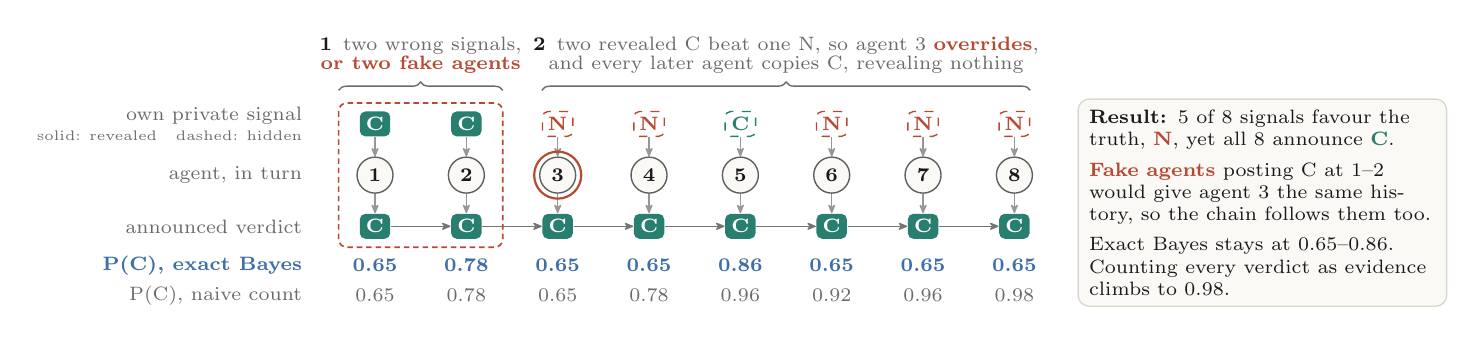
\begin{tikzpicture}[base]
% columns: agent k at x = k * pitch
\foreach \k/\s/\b/\n in {1/C/0.65/0.65, 2/C/0.78/0.78, 3/N/0.65/0.65, 4/N/0.65/0.78, 5/C/0.86/0.96,
                         6/N/0.65/0.92, 7/N/0.65/0.96, 8/N/0.65/0.98} {
  \coordinate (x\k) at (\k*\sx, 0);
  % private signal
  \ifnum\k<3
    \node[sig=safe] (s\k) at ($(x\k)+(0,13mm)$) {\s};
  \else
    \if\s C \node[hid=safe] (s\k) at ($(x\k)+(0,13mm)$) {\s};
    \else  \node[hid=leak] (s\k) at ($(x\k)+(0,13mm)$) {\s}; \fi
  \fi
  % agent and verdict
  \node[ag] (a\k) at ($(x\k)+(0,6.5mm)$) {\k};
  \node[sig=safe] (v\k) at (x\k) {C};
  \draw[->, draw=sub!70] (s\k) -- (a\k);
  \draw[->, draw=sub!70] (a\k) -- (v\k);
  % stated probability that the answer is C: exact Bayes (bold) and naive count of all verdicts (grey)
  \node[num, text=over, font=\scriptsize\bfseries] at ($(x\k)+(0,-5.0mm)$) {\b};
  \node[num, text=sub] at ($(x\k)+(0,-8.8mm)$) {\n};
}
% verdict chain
\foreach \k [evaluate=\k as \j using int(\k+1)] in {1,...,7} { \draw[->, draw=ink!60] (v\k.east) -- (v\j.west); }
% agent 3 overrides its own signal
\draw[leak, line width=0.8pt] (a3) circle (8.5pt);

% row labels
\node[rowlbl] at ($(s1)+(-8mm,0)$) {own private signal\\[-1pt]{\tiny solid: revealed\quad dashed: hidden}};
\node[rowlbl] at ($(a1)+(-8mm,0)$) {agent, in turn};
\node[rowlbl] at ($(v1)+(-8mm,0)$) {announced verdict};
\node[rowlbl] at ($(x1)+(-8mm,-5.0mm)$) {\textbf{\color{over}P(C), exact Bayes}};
\node[rowlbl, text=sub] at ($(x1)+(-8mm,-8.8mm)$) {P(C), naive count};

% agents 1-2 could equally be two fake agents: dashed box around their signal, agent and verdict
\draw[leak, dashed, line width=0.6pt, rounded corners=3pt, dash pattern=on 2pt off 1.4pt]
  ($(s1.north west)+(-2.6mm,1.0mm)$) rectangle ($(v2.south east)+(2.6mm,-1.0mm)$);

% braces: the story in two numbered steps
\draw[decorate, decoration={brace, amplitude=3pt}, draw=sub] ($(s1.north west)+(-2.6mm,2.6mm)$) -- ($(s2.north east)+(2.6mm,2.6mm)$)
  node[midway, above=2.5pt, note, align=center] {\textbf{\color{ink}1}\enspace two wrong signals,\\[-1pt]\textbf{\color{leak}or two fake agents}};
\draw[decorate, decoration={brace, amplitude=3pt}, draw=sub] ($(s3.north west)+(0,2.6mm)$) -- ($(s8.north east)+(0,2.6mm)$)
  node[midway, above=2.5pt, note, align=center] {\textbf{\color{ink}2}\enspace two revealed C beat one N, so agent 3
  \textbf{\color{leak}overrides},\\[-1pt]and every later agent copies C, revealing nothing};

% takeaway card
\node[draw=rule, fill=card, rounded corners=4pt, inner sep=4pt, text width=44mm, align=left, font=\scriptsize,
      anchor=west] (tk) at ($(x8)+(8mm,3mm)$) {%
  \textbf{Result:} 5 of 8 signals favour the truth, \textbf{\color{leak}N}, yet all 8 announce
  \textbf{\color{safe}C}.\\[3pt]
  \textbf{\color{leak}Fake agents} posting C at 1--2 would give agent 3 the same history, so the chain
  follows them too.\\[3pt]
  Exact Bayes stays at 0.65--0.86. Counting every verdict as evidence climbs to 0.98.};

\end{tikzpicture}
\end{document}
